%\section{Humanoid Path Planner (HPP)}

The complex motion of leaning forward and picking the hose from the floor pose several problems.
%
First auto collisions are possible between the femurs and the hip joints due to the structure design of the HRP-$2$ humanoid robot.
%
Second a reactive approach does not find a good solution because of local minima.
%
For these reasons we employed the Humanoid Path Planner (HPP) to compute the motion for picking the hose from the floor.
%
This exact same versatile library we used to plan the contact point on the multi-contact climbing stair motion in Chap.~\ref{chap:multicontact}.
%
As a reminder HPP, \cite{hpp} is an open source software able to compute a collision-free path from a given starting robot configuration to a goal one.
%
This path is subject to a set of constraints such as balance conditions, a particular posture for specific DOF(s), etc.
%
It is also able to randomly search for a robot configuration satisfying a set of desired constraints, including environment and self-collision checking.
%
For picking the fire hose from the floor, first we search for a robot configuration with the following constraints:
%
\vspace{0.7mm}
\begin{list}{\arabic{ass}.}{%
		\usecounter{ass}%
		\setlength{\topsep}{2pt}%
		\setlength{\itemsep}{0pt}%
		\setlength{\parsep}{0pt}%
		\setlength{\labelwidth}{1.5em}%
		\setlength{\leftmargin}{1.5em}%
		\setlength{\labelsep}{0.5em}%
	}
%
\item The robot's center of mass must be at the center of the support polygon.
%
\item Both of the robot's feet should keep in contact with the floor.
%
\item The left wrist height must be such that it can reach the hose without colliding with the floor.
%
\item The robot's waist orientation is fixed and facing forward.
%
\end{list}


Furthermore, we use the robot's half sitting configuration to limit the results from the random search to configurations that satisfy:
%
\vspace{-1mm}
\begin{equation*}
\mathbf{q}_{\text{res}} = \mathbf{q}_{\text{rand}}' + \big( \mathbf{I}_{\text n} - \mathbf{J}^{+}\mathbf{J}(\mathbf{q}_{\text{rand}}')(\mathbf{q}_{\text{hs}} - \mathbf{q}_{\text{rand}}') \big)
\vspace{-1mm}
\end{equation*}
%
where $\mathbf{q}_{\text{rand}}'$ is the projection of a random configuration $\mathbf{q}_{\text{rand}}$ into the constrained space, $\mathbf{q}_{\text{hs}}$ is the robot's half sitting configuration, $\mathbf J$ is the Jacobian of the robot tasks and $\mathbf{I}_{\text n}$ is the identity matrix of $n\times n$, and $\mathbf{q}_{\text{res}}$ is the projection of $\mathbf{q}_{\text{hs}}$ on the constrained tangent space at $\mathbf{q}_{\text{rand}}'$.
%
The desired robot configuration is the projection of $\mathbf{q}_{\text{res}}$ into the constrained space $\mathbf{q}_{\text{res}}'$. 
%
%
After obtaining the picking configuration, we compute two free collision paths, the first starting at the half sitting configuration and finishing on $\mathbf{q}_{\text{res}}'$, and the second starting at $\mathbf{q}_{\text{res}}'$ and going back to the half sitting configuration, both of them subject to constraints 1, 2 and 4 during the whole path.
%
From the obtained path we extract the information of the robot's center of mass position, both feet's position and orientation, and the robot's configuration angles.
%
These information will be use by an inverse kinematic framework for redundant robots that prioritizes robot tasks by projecting low priority tasks into the kernel of high priority tasks \cite{mansard:icar:09}.
%
\begin{figure}[t]
 \centering
 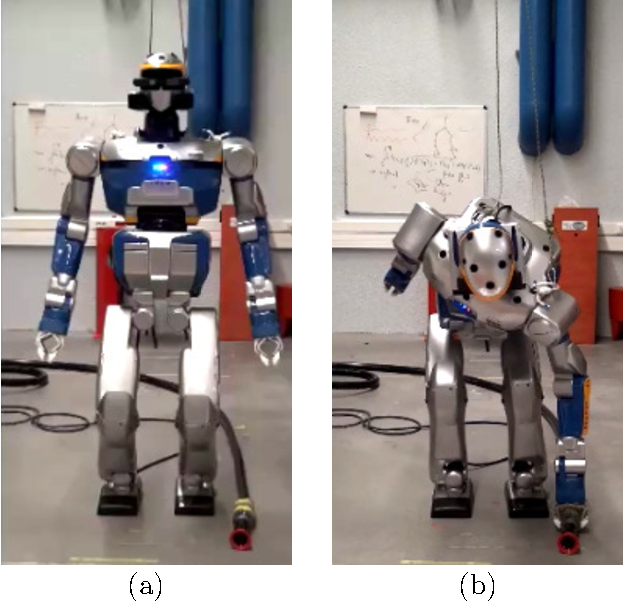
\includegraphics[height=0.40\textwidth]{./figures/Pick_2pics.pdf}
 \vspace{-3mm}
 \caption{Snapshots of the experiment on the HRP-$2$ robot picking a fire hose from the floor.}
 \label{exp_pick}
% \vspace{-5mm}
\end{figure}
